%%%%%%%%%%%%%%%%%%%%%%%%%%%%%%%%%%%%%%%%%%%%%%%%%%%%%%%%%%%%%%%%%%%%%%%%%%%%%%%
% File: documentation.tex
% Encoding: utf8
% Project: VYPe - Conversion from regular expressions to finite automata
% Authors:
%     Libor Polčák, xpolca03@stud.fit.vutbr.cz
%     Petr Zemek, xzemek02@stud.fit.vutbr.cz
% Description: Project documentation
%%%%%%%%%%%%%%%%%%%%%%%%%%%%%%%%%%%%%%%%%%%%%%%%%%%%%%%%%%%%%%%%%%%%%%%%%%%%%%%

% Configuration
\documentclass[10pt, notitlepage]{article}

% Style
\usepackage{documentation}

%%%%%%%%%%%%%%%%%%%%%%%%%%%%%%%% Document info %%%%%%%%%%%%%%%%%%%%%%%%%%%%%%%%
\title{Demonstrační program - převod regulárního výrazu na konečný automat}
\project{Projekt do předmětu Výstavba překladačů}

\author{
Libor Polčák, xpolca03@stud.fit.vutbr.cz \\
Petr Zemek, xzemek02@stud.fit.vutbr.cz \\
}

%%%%%%%%%%%%%%%%%%%%%%%%%%%%%%%% Main document %%%%%%%%%%%%%%%%%%%%%%%%%%%%%%%%
\begin{document}

% Title page
\maketitle

% Page numbering
\setcounter{page}{2}

%%%%%%%%%%%%%%%%%%%%%%%%%%%%%%%%%%%% Text %%%%%%%%%%%%%%%%%%%%%%%%%%%%%%%%%%%%%

\section{Úvod}
\label{sec:Introduction}

Tento dokument obsahuje projektovou dokumentaci k~projektu \uv{Demonstrační
program - převod regulárního výrazu na konečný automat}, realizovaný v~rámci
předmětu \uv{VYPe - Výstavba překladačů}.

Jak již název napovídá, jedná se vizuální pomůcku při výkladu algoritmů pro
převod regulárních výrazů na konečné automaty. Našim cílem bylo vyvinout
jednoduchou a přehlednou aplikaci, která by byla vhodná právě k~tomuto účelu.

V~sekci \ref{sec:Installation} je popsán způsob instalace aplikace a seznam
všech nutných prerekvizit nutných pro její spuštění. V~následující sekci
\ref{sec:AppDesc} se nachází obecný popis aplikace a jejího ovládání. Sekce
\ref{sec:Design} popisuje návrh a implementaci aplikace. Poslední sekce
\ref{sec:Conclusion} obsahuje shrnutí naší práce na projektu a jeho zhodnocení.

\section{Instalace a spuštění aplikace}
\label{sec:Installation}

Instalace spočívá v~rozbalení archivu do libovolného adresáře. Pro spuštění
aplikace je třeba nainstalovat následující software:

\begin{itemize}
	\item \texttt{python >= 2.5} (\url{http://www.python.org/})
	\item \texttt{wxPython >= 2.8} (\url{http://www.wxpython.org/})
	\item \texttt{graphviz >= 2.20} (\url{http://www.graphviz.org/})
\end{itemize}

Aplikace se pak spouští příkazem \texttt{python vype.py} (předpokladem je
správně nastavená proměnná \texttt{PATH}). Aplikace byla testována v~systémech
GNU/Linux (distribuce Debian Unstable a Ubuntu Hardy) a MS Windows XP.

\section{Popis aplikace}
\label{sec:AppDesc}

Aplikace slouží pro výuku a demonstrační účely. Hlavním smyslem aplikace je
ukázat uživateli, jakým způsobem se provádí převod libovolného regulárního
výrazu na ekvivaletní konečný automat. Aplikace je vhodná i pro výuku ve
větších skupinách, protože umožňuje snadnou volbu velikosti písma.

\begin{figure}[h]
	\begin{center}
		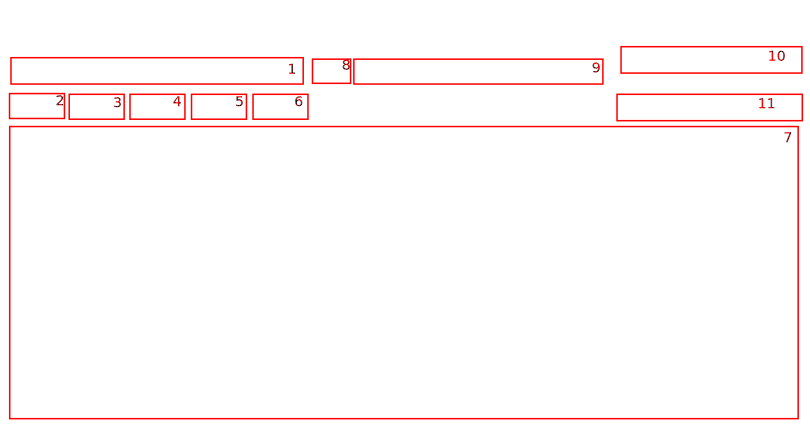
\includegraphics[width=\textwidth,keepaspectratio]{include/gui}
	\end{center}
	\caption{Grafické uživatelské rozhraní.}
	\label{fig:GUI}
\end{figure}

Na obrázku \ref{fig:GUI} je zachyceno hlavní okno aplikace. Skládá se z~těchto
prvků:

\begin{itemize}
	\item 1 je pole pro zadání vstupního regulárního výrazu,

	\item 2 je tlačítko pro zpracování vstupního regulárního výrazu,

	\item 3 je tlačítko provádějící skok na první krok převodu,

	\item 4 je tlačítko pro přesun na předcházející krok převodu,

	\item 5 je tlačítko pro přesun na následující krok převodu,

	\item 6 je tlačítko provádějící skok na poslední krok převodu,

	\item 7 je plocha, do kterého se vykresluje konečný automat vytvořený
		v~aktuálním kroku převodu,

	\item 8 obsahuje pořadové číslo aktuálně zobrazeného kroku převodu a jejich
		celkový počet,

	\item 9 obsahuje regulární výraz, který odpovídá právě zobrazenému
		konečnému automatu,

	\item 10 umožňuje uživateli zvětšovat a zmenšovat písmo použité v~prvcích
		1, 7, 8 a 9.

	\item 11 dovoluje uživateli změnit barvu vyznačených částí automatu, které
		prodělaly oproti předchozímu kroku změnu.

\end{itemize}

Okno je aplikace je možné zvětšovat a zmenšovat. Grafická reprezentace automatu
se však vždy zobrazuje tak, aby se vešla do prostoru 7. Pokud jsou rozměry
obrázku větší než je velikost plochy 7, je obrázek zmenšen tak, aby se do plochy
vešel.

Kromě navigačních tlačítek je možné se mezi jednotlivými kroky pohybovat pomocí
klávesových zkratek. \texttt{Šipka doprava} a \texttt{nahoru} zobrazí
následující krok, \texttt{šipka doleva} a \texttt{dolů} krok předchozí. Klávesy
\texttt{Page Up} a \texttt{End} zobrazí poslední krok převodu regulárního výrazu
na automat, zatímco klávesy \texttt{Page Down} a \texttt{Home} ukáží krok první.

Uživatel má možnost zadat libovolný regulární výraz nad abecedou obsahující
všechny znaky dostupné v~kódování Unicode. Tento přístup byl zvolen proto, aby
uživatel nebyl při zápisu regulárních výrazů nijak zásadně omezován a mohl
používat znaky s~diakritikou, z~jiných abeced apod.

Jednoduchý (nesložený) regulární výraz je možné zapsat následujícím způsobem:

\begin{itemize}
	\item \texttt{\textbackslash 0} reprezentuje prázdnou regulární množinu,

	\item \texttt{\textbackslash e} reprezentuje prázdný řetězec,

	\item Libovolný znak ze sady Unicode (kromě znaků \texttt{\textbackslash},
	\texttt{(}, \texttt{)}, \texttt{+} a \texttt{*}, které jsou použity jako
	metaznaky) reprezentuje daný symbol.
\end{itemize}

Za předpokladu, že \texttt{u} a \texttt{v} jsou regulární výrazy, je možné
skládat složitější regulární výrazy takto:

\begin{itemize}
	\item \texttt{u+v} reprezentuje sjednocení regulárních výrazů \texttt{u} a
		\texttt{v},

	\item \texttt{uv} reprezentuje konkatenaci regulárních výrazů \texttt{u} a
		\texttt{v},

	\item \texttt{u*} reprezentuje iteraci regulárního výrazu \texttt{u}.
\end{itemize}

Pomocí závorek \texttt{(} a \texttt{)} je možné měnit prioritu operací nad
regulárními výrazy (standardně má iterace přednost před konkatenací a ta má
přednost před sjednocením).

Pro použití metaznaků jako obyčejných znaků lze využít následující \uv{escape
sekvence}:

\begin{itemize}

	\item \texttt{\textbackslash \textbackslash} reprezentuje symbol
		\texttt{\textbackslash},

	\item \texttt{\textbackslash (} reprezentuje symbol \texttt{(},

	\item \texttt{\textbackslash )} reprezentuje symbol \texttt{)},

	\item \texttt{\textbackslash +} reprezentuje symbol \texttt{+},

	\item \texttt{\textbackslash *} reprezentuje symbol \texttt{*}.
\end{itemize}

Po zpracování zadaného regulárního výrazu umožňuje aplikace uživateli volně
procházet jednotlivými kroky tvorby automatu a to včetně návratu k~předchozím
krokům. V~každém kroku převodu je také zobrazeno, kterému regulárnímu podvýrazu
právě zobrazený automat odpovídá.

Aby se uživatel neztratil v~označení jednotlivých stavů automatů při
vytváření složitějších automatů z~jednodušších, zůstává označení stavů stejné,
jaké bylo v~původních automatech.

Pokud při běhu programu nastane nějaká chyba, jako je například špatně zadaný
regulární výraz, nemožnost vytvoření grafické reprezentace automatu apod., je
uživateli zobrazeno chybové okno, ve kterém jsou uživateli sděleny bližší
informace o~chybě.

\section{Návrh a implementace}
\label{sec:Design}

Jako implementační jazyk jsme zvolili
\texttt{Python}\footnote{\url{http://www.python.org/}}, a to z~důvodu toho, že
jsme s~vytvářením aplikací v~tomto jazyce již měli zkušenosti.
Pro usnadnění spolupráce při vytváření projektu a zjednodušení testování jsme
v~rámci návrhu aplikace dekomponovali na několik částí. První část se týká
regulárních výrazů. Zde se nachází reprezentace regulárních výrazů, která je
vhodná pro následné zpracování (převod na konečný automat) a syntaktický
analyzátor regulárních výrazů. Popis implementace této části se nachází
v~sekci \ref{sec:ImplRegExps}.

Druhou částí jsou konečné automaty. Zde se nachází jejich vhodná reprezentace a
možnost skládání složitějších automatů z~jednodušších částí. Jelikož jsme se
rozhodli pro vyobrazení automatů použít externí program
\texttt{graphviz}\footnote{\url{http://www.graphviz.org/}} (z~důvodu kvality
výsledných grafických schémat automatů), tak tato část dále obsahuje převod
vytvořených automatů na textovou reprezentaci vhodnou pro převod na obrázek a
samotný převod této reprezentace na obrázek pomocí zmíněné aplikace. Popis
implementace této části se nachází v~sekci \ref{sec:ImplAutomata}.

Konečně, poslední částí je samotné grafické uživatelské rozhraní, které využívá
předcházející části. Zde jsme použili grafickou knihovnu
\texttt{wxPython}\footnote{\url{http://www.wxpython.org/}}, kterou jsme zvolili
z~důvodu její přenositelnosti na různé systémy a důvodu předházejících
zkušeností s~touto knihovnou. Grafické uživatelské rozhraní jsme vytvořili
pomocí nástroje \texttt{wxGlade}\footnote{http://wxglade.sourceforge.net/}. Pro
tuto část v~této dokumentaci nejsou žádné další detaily (vše je dostatečně
popsáno v~sekci \ref{sec:AppDesc}).

Implementační záležitosti, které se nedostaly do žádné z~předchozích částí, se
nachází v~sekci \ref{sec:ImplOthers}.

\subsection{Regulární výrazy}
\label{sec:ImplRegExps}

Modul \emph{regexp} obsahuje hierarchii tříd reprezentující regulární výrazy.
Bázová třída je pojmenovaná \emph{RegExp} a obsahuje výchozí implementaci metod,
které jsou obvykle v~odvozených třídách předefinovány. Jedná se o~konstruktor,
metody pro určení rovnosti a nerovnosti dvou regulárních výrazů a metodu pro
textovou reprezentaci prostřednictvím znakové sady Unicode.

Odvozené třídy vycházejí z~definice regulárních množin. Je k~dispozici třída
\emph{EmptySetRegExp}, \emph{EpsilonRegExp}, které reprezentují regulární výrazy
$\emptyset$, respektive $\varepsilon$. Třída \emph{SingleSymbolRegExp} pak
reprezentuje regulární výraz odpovídající jednomu symbolu ze vstupní abecedy.
Třída je schopná uchovávat jakýkoliv znak, jenž je možné v~jazyce Python
reprezentovat pomocí bázové třídy \emph{basestring}.

Dále jsou v~hierarchii třídy umožňující skládat složitější regulární výrazy
z~jednoho, případně dvou jiných regulárních výrazů. První z~nich je třída
\emph{UnionRegExp}, která umožňuje provést sjednocení dvou regulárních výrazů.
Další z~nich je třída \emph{ConcatRegExp} umožňující konkatenaci dvou
regulárních výrazů. Třída \emph{IterRegExp} pak reprezentuje iteraci nad jedním
regulárním výrazem. Pro snadnou reprezentaci regulárního výrazu tak, jak byl
zadán před parsováním, je součástí hierarchie také třída pro reprezentaci jednoho
regulárního výrazu v~závorkách pojmenovaná \emph{BracketsRegExp}.

Modul \emph{regexp\_parser} slouží k~převodu textového řetězce reprezentujícího
regulární výraz na jeho reprezentaci pomocí hierarchie výše popsaných tříd.
Tento parser pracuje s~abecedou $\Sigma$, která obsahuje všechny znaky dostupné
v~kódování Unicode, na základě gramatiky $G_1 = (N, T, S, P)$, kde:

\begin{itemize}
	\item $N = \{S, U, K, I\}$,

	\item $T = \{(, ), +, *\} \cup  \Sigma \cup \{\varepsilon, \emptyset\}$

	\item $P = \{S \rightarrow S+U | U, U \rightarrow UK | K, K \rightarrow K* |
		I, I \rightarrow (S) | \emptyset | \varepsilon\} \cup \{I \rightarrow x |
		x \in \Sigma\}$
\end{itemize}

Gramatika $G_1$ však obsahuje levou rekurzi, kterou odstraníme vytvořením
evivalentní gramatiky $G_2 = (N, T, S, P)$. Tato gramatika je ta, ze kterou
parser skutečně pracuje.

\begin{itemize}
	\item $N = \{S, S', U, U', K, K', I\}$,

	\item $T = \{(, ), +, *\} \cup  \Sigma \cup \{\varepsilon, \emptyset\}$

	\item $P = \{S \rightarrow US', S' \rightarrow \varepsilon | +US', U
		\rightarrow KU', U' \rightarrow \varepsilon | KU', K \rightarrow IK', K'
		\rightarrow \varepsilon | *K', I \rightarrow (S) | \emptyset |
		\varepsilon\} \cup \{I \rightarrow x | x \in \Sigma\}$
\end{itemize}

Parser je založen na metodě rekurzivního sestupu. Tedy obsahuje funkce, které
odpovídají jednotlivým nonterminálům gramatiky $G_2$. V~těchto funkcích se pak
aplikují pravidla gramatiky $G_2$, ve kterých je daný nonterminál na levé
straně. Současně se vytvoří instance třídy příslušející k~danému podstromu
derivačního stromu.

\subsection{Automaty}
\label{sec:ImplAutomata}

Modul \emph{nfas} obsahuje bázovou abstraktní třídu \emph{NFA} pro všechny
ostatní automaty. Automaty jsou obecně nedeterministické. Vnitřně jsou
reprezentováný algebraicky, čili je uchováván seznam (množina) stavů, počáteční
stav, seznam (množina) koncových stavů a seznam přechodů (seznam trojic ---
stav, ze kterého se přechází, symbol a stav, do kterého se přechází).
V~rámci zjednodušení implementace má každý automat nejvýše jeden koncový stav.

Jak již bylo popsáno v~sekci \ref{sec:ImplRegExps}, tak při převodu regulárních
výrazů na konečné automaty jsou potřeba následující trídy. Třída
\emph{EmptySetNFA} reprezentuje konečný automat korespondující k~regulárnímu
výrazu $\emptyset$. Jeho grafické vyobrazení\footnote{Uživatel má možnost
nastavení výsledné barvy automatů a zvýraznění změněných částí. Obrázkům
automatů v~této dokumentaci byla ponechána pouze černá barva, která je pro
základní představu, jak tyto automaty vypadjí, dostačující.} je na Obrázku
\ref{fig:EmptySetNFA}.

\begin{figure}[h]
	\begin{center}
		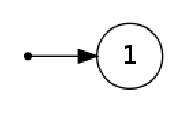
\includegraphics[width=2cm,keepaspectratio]{include/emptysetnfa}
	\end{center}
	\caption{Vyobrazení instance třídy \emph{EmptySetNFA}.}
	\label{fig:EmptySetNFA}
\end{figure}

Třída \emph{SingleSymbolNFA} reprezentuje automat přijímající jazyk
obsahující jeden symbol --- ať již se jedná o~symbol ze vstupní abecedy či
o~prázný řetězec \emph{epsilon}. Grafické vyobrazení instance této třídy,
korespondující k~regulárnímu výrazu $a$, je na obrázku \ref{fig:SingleSymbolNFA}.

\begin{figure}[h]
	\begin{center}
		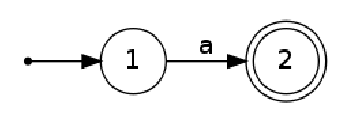
\includegraphics[width=4cm,keepaspectratio]{include/singlesymbolnfa}
	\end{center}
	\caption{Vyobrazení instance třídy \emph{SingleSymbolNFA}.}
	\label{fig:SingleSymbolNFA}
\end{figure}

Po těchto jednoduchých automatech následují kompozice automatů. Třída
\emph{ConcatNFA} reprezentuje konkatenaci dvou regulárních výrazů (automatů).
Vznikne z~nich tak, že se koncový stav prvního automatu nahradí za nekoncový
a spojí se epsilon přechodem s~původním počátečním stavem druhého automatu
(který ve výsledném automatu již počátečním stavem není). Ukázka konkatenace
dvou automatů, kde první z~nich koresponduje k~regulárnímu výrazu $a$ a druhý
koresponduje k~regulárnímu výrazu $b$, je na obrázku \ref{fig:ConcatNFA}.

\begin{figure}[h]
	\begin{center}
		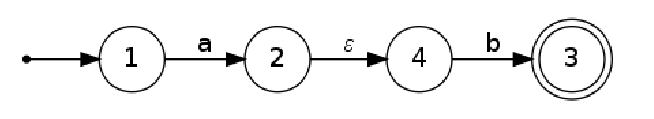
\includegraphics[width=8cm,keepaspectratio]{include/concatnfa}
	\end{center}
	\caption{Vyobrazení instance třídy \emph{ConcatNFA}.}
	\label{fig:ConcatNFA}
\end{figure}

Třída \emph{UnionNFA} reprezentuje sjednocení dvou regulárních výrazů
(automatů). Vznikne z~nich tak, že se vytvoří nový počáteční a koncový stav,
z~počátečního stavu se svedou epsilon přechody do počátečních stavů původních
automatů a z~koncových stavů původních automatů se svede epsilon přechod do
nově vytvořeného koncového stavu. Ukázka sjednocení dvou automatů, kde první
z~nich koresponduje k~regulárnímu výrazu $a$ a druhý koresponduje
k~regulárnímu výrazu $b$, je na obrázku \ref{fig:UnionNFA}.

\begin{figure}[h]
	\begin{center}
		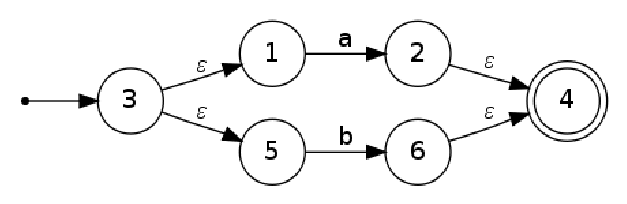
\includegraphics[width=8cm,keepaspectratio]{include/unionnfa}
	\end{center}
	\caption{Vyobrazení instance třídy \emph{UnionNFA}.}
	\label{fig:UnionNFA}
\end{figure}

Poslední třídou je třída \emph{IterNFA}, která reprezentuje iteraci regulárního
výrazu (automatu). Vznikne z~automatu tak, že se vytvoří nový počáteční a
koncový stav. Z~nového počátečního stavu se vyvede epsilon přechod do
počátečního stavu původního automatu a koncového stavu nového automatu.
Z~koncového stavu původního automatu se vyvede epsilon přechod do koncového
stavu nového automatu a do počátečního stavu původního automatu. Ukázka iterace
automatu, který koresponduje k~regulárnímu výrazu $a^{*}$, je na obrázku
\ref{fig:IterNFA}.

\vspace*{-4cm}
\begin{figure}[h]
	\begin{center}
		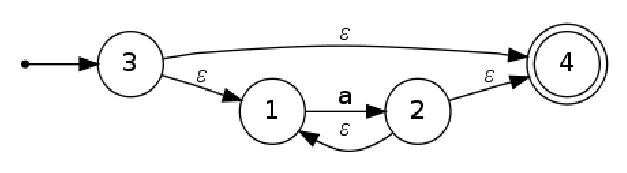
\includegraphics[width=8cm,keepaspectratio]{include/iternfa}
	\end{center}
	\caption{Vyobrazení instance třídy \emph{IterNFA}.}
	\label{fig:IterNFA}
\end{figure}

\pagebreak
Pro převod automatů na textovou reprezentaci vhodnou pro převod na obrázek
slouží modul \emph{nfa2dot}. Funkce \emph{convertNFAtoDOT()} z~tohoto
modulu provádí převod předané instance automatu na reprezentaci v~jazyce
\emph{DOT}, který lze programem \texttt{dot} (je součástí \texttt{graphviz}u)
převést na obrázek. Převod je realizován postupným procházením všech stavů a
přechodů automatů a vytváření textové reprezentace. Níže je vidět textová
reprezentace automatu z~obrázku \ref{fig:IterNFA}.

\begin{verbatim}
    digraph finite_state_machine {
        node [shape = point]; S3;
        node [shape = circle]; 3;
        node [shape = doublecircle]; 4;
        node [shape = circle]; 1;
        node [shape = circle]; 2;
        S3 -> 3 [ label = "" ];
        1 -> 2 [ label = "a" ];
        3 -> 1 [ label = "e", fontname = "Times-Italic" ];
        3 -> 4 [ label = "e", fontname = "Times-Italic" ];
        2 -> 4 [ label = "e", fontname = "Times-Italic" ];
        2 -> 1 [ label = "e", fontname = "Times-Italic" ];
    }
\end{verbatim}

Jelikož označení stavů musí být z~důvodu bezpečnosti vytváření kombinací
automatů unikátní, tak pro jejich přejmenování na čitelná jména stavu slouží
funkce \emph{renameStates()} z~modulu \emph{dot}. Pomocí této funkce lze
přejmenovat všechny stavu zadaného automatu (z~jejich textové reprezentace)
podle zadaného generátoru (v~aplikaci je použit generátor přirozených čísel).
Implementace této funkce je založena na postupném procházení řádků textové
reprezentace, uchovávání si mapování mezi původními a novými označeními stavů.
Toto mapování se pro zachování označení stavů mezi jednotlivými automaty
předává funkci jako vstupně/výstupní parametr.

Konečně, pro konverzi textové reprezentace automatu na obrázek slouží funkce
\emph{createImage()} z~modulu \emph{dot2img}. Ta volá externí program
\texttt{dot} (součástí \texttt{graphviz}u), který na zadaném umístění vytvoří
obrázek automatu v~zadaném formátu (v~aplikaci využíváme formát PNG).
K~zavolání externího programu a komunikace s~ním je použit modul
\emph{subprocess} ze standardní pythonovské knihovny.

\subsection{Ostatní}
\label{sec:ImplOthers}

Z~výkonnostních důvodů nejsou po analýze regulárního výrazu vytvořeny obrázky
příslušející jednotlivým automatům, ale je využito odloženého zpracování, kdy
se obrázek automatu příslušející určitému regulárnímu výrazu vytváří až ve
chvíli, kdy má být zobrazen. Poté je výsledek uložen do paměti a použit
v~případě budoucího zobrazení (není tedy třeba znovu provádět převod daného
automatu na obrázek).

\section{Závěr}
\label{sec:Conclusion}

Během vytváření aplikace jsme využívali systém pro správu verzí
\texttt{subversion}\footnote{\url{http://www.subversion.tigris.org/}}.
Komunikace během vypracování projektu byla osobní, jelikož oba bydlíme ve
stejném pokoji na studentských kolejích. Tato skutečnost nám velmi usnadnila
spolupráci na projektu.

Testována byla jak aplikační logika (190 automatizovaných testů s~využitím
modulu \texttt{unittest} --- lze je spustit pomocí \texttt{python tester.py}),
tak aplikační rozhraní. V~rámci testování přenositelnosti jsme aplikaci úspěšně
vyzkoušeli na systémech GNU/Linux a MS Windows XP.

Při návrhu a implementaci bylo naším cílem vytvořit fungující a rozšiřitelnou
aplikaci, která by plnila svůj účel. S~výsledkem jsme spokojeni a věříme, že
najde uplatnění jako učební pomůcka.
Co se týče možných rozšíření, tak jednou z~možností by bylo přidání
reprezentace regulárních výrazů v~podobě syntaktického stromu, která by jasněji
vyjadřovala postup při konstrukci jednotlivých automatů a jejich spojování do
větších celků.

\end{document}

%%%%%%%%%%%%%%%%%%%%%%%%%%%%%%%%%%%%%%%%%%%%%%%%%%%%%%%%%%%%%%%%%%%%%%%%%%%%%%%
% vim: syntax=tex
%%%%%%%%%%%%%%%%%%%%%%%%%%%%%%%%%%%%%%%%%%%%%%%%%%%%%%%%%%%%%%%%%%%%%%%%%%%%%%%
